\documentclass{standalone}
\usepackage{tikz}
\usepackage{amsmath}
\usetikzlibrary{matrix}
\usetikzlibrary {shapes.geometric}
\usetikzlibrary {arrows.meta}
\begin{document}
    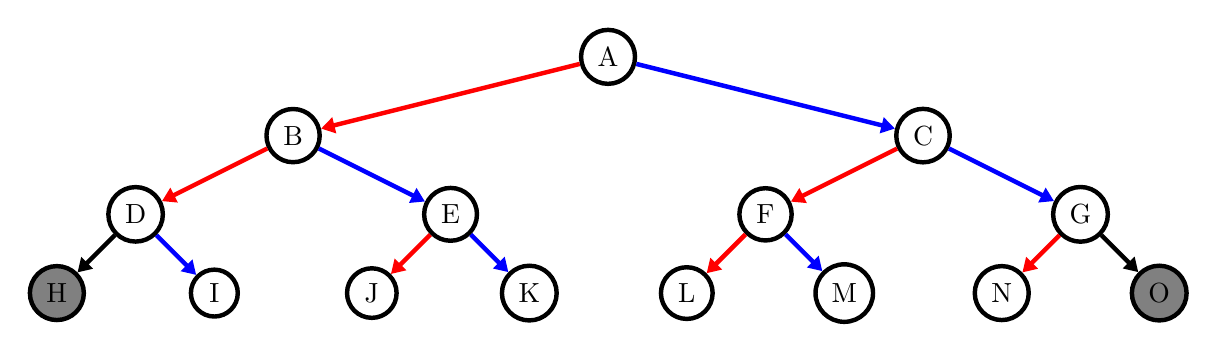
\begin{tikzpicture}[ultra thick]

        %\draw [help lines] (0,0) grid (16,16); 

        \path   (8,10)  node (a) [circle,draw] {A}
                (4,9) node (b) [circle,draw] {B}
                (12,9) node (c) [circle,draw] {C}
                (2,8) node (d) [circle,draw] {D}
                (6,8) node (e) [circle,draw] {E}
                (10,8) node (f) [circle,draw] {F}
                (14,8) node (g) [circle,draw] {G}
                (1,7) node (h) [circle,draw,fill=gray] {H}
                (3,7) node (i) [circle,draw] {I}
                (5,7) node (j) [circle,draw] {J}
                (7,7) node (k) [circle,draw] {K}
                (9,7) node (l) [circle,draw] {L}
                (11,7) node (m) [circle,draw] {M}
                (13,7) node (n) [circle,draw] {N}
                (15,7) node (o) [circle,draw,fill = gray] {O};

                
            
        \draw[arrows = -{Triangle[open,angle=60:2mm,fill = red]},red]  (node cs: name =a ) -- (node cs:name =b);
        \draw[arrows = -{Triangle[open,angle=60:2mm,fill = blue]},blue] (node cs: name =a ) -- (node cs:name =c);
        \draw[arrows = -{Triangle[open,angle=60:2mm,fill = red]},red] (node cs: name =b ) -- (node cs:name =d);
        \draw[arrows = -{Triangle[open,angle=60:2mm,fill = blue]},blue] (node cs: name =b ) -- (node cs:name =e);
        \draw[arrows = -{Triangle[open,angle=60:2mm,fill = red]},red] (node cs: name =c ) -- (node cs:name =f);
        \draw[arrows = -{Triangle[open,angle=60:2mm,fill = blue]},blue] (node cs: name =c ) -- (node cs:name =g);
        \draw[arrows = -{Triangle[open,angle=60:2mm,fill = black]},black] (node cs: name =d ) -- (node cs:name =h);
        \draw[arrows = -{Triangle[open,angle=60:2mm,fill = red]},red] (node cs: name =e ) -- (node cs:name =j);
        \draw[arrows = -{Triangle[open,angle=60:2mm,fill = red]},red] (node cs: name =f ) -- (node cs:name =l);
        \draw[arrows = -{Triangle[open,angle=60:2mm,fill = red]},red] (node cs: name =g) -- (node cs:name =n);
        \draw[arrows = -{Triangle[open,angle=60:2mm,fill = blue]},blue] (node cs: name =d ) -- (node cs:name =i);
        \draw[arrows = -{Triangle[open,angle=60:2mm,fill = blue]},blue] (node cs: name =e ) -- (node cs:name =k);
        \draw[arrows = -{Triangle[open,angle=60:2mm,fill = blue]},blue] (node cs: name =f) -- (node cs:name =m);
        \draw[arrows = -{Triangle[open,angle=60:2mm,fill = black]},black] (node cs: name =g ) -- (node cs:name =o);
        
    \end{tikzpicture}

\end{document}